% !TEX root = ../paper.tex
To fairly evaluate \textit{Laserlight} and \textit{MTV}, I incorporate their own data sets and empirically evaluate them against \textit{naive mixture encoding} under their own applications.

\tinysection{Data Sets}
Specifically, I choose \textit{Mushroom} data set used in \textit{MTV}~\cite{DBLP:journals/tkdd/MampaeyVT12} which is obtained from FIMI dataset repository and U.S. Census data on Income or simply \textit{Income} data set, which is downloaded from IPUMS-USA at \textit{https://usa.ipums.org/usa/} and used in \textit{Laserlight}~\cite{DBLP:journals/pvldb/GebalyAGKS14}.
The basic statistics of the data sets are given in Table~\ref{table:extendeddatasummary}.

\begin{table}[h!]
\centering
\bfcaption{Data Sets of Alternative Applications}
\label{table:extendeddatasummary}
{\small \centering
\begin{tabular}{c c c}
\toprule
Statistics & Income & Mushroom \\
\midrule
\# Distinct data tuples & 777493 & 8124\\
\midrule
\# Features per tuple & 9 & 21\\
\midrule
Feature Binary-valued? & no& no\\
\midrule
\# Distinct features & 783 & 95\\
\midrule
Binary Classification Feature & $>100,000$? & Edibility\\
\midrule
Assumed data tuple multiplicity & 1 & 1\\
\bottomrule
\end{tabular}
}
\end{table}

\subsection{Experiments}
\label{sec:evaluatingalternativeapplicationsexperiments}
All experiments involving \textit{Laserlight} and \textit{MTV} will be evaluated under their own Error measures and data sets, unless otherwise stated.
The experiments are organized as follows: First, we establish baselines by evaluating classical \textit{Laserlight} and \textit{MTV} on their original data; Then we show that classical \textit{Laserlight} and \textit{MTV} can be generalized to partitioned data and that the generalization improves on their Error measures and also runtime; At last, we compare their generalized versions with \textit{naive mixture encoding} to show that \textit{naive mixture encoding} is a reasonable alternative.% in terms of run time and Error.

\subsubsection{Error Measures}
We first explain how \textit{naive mixture encoding} is evaluated based on Error defined by \textit{Laserlight} and \textit{MTV}.

\tinysection{Evaluating Naive Encoding on Laserlight Error}
Algorithm \textit{Laserlight} summarizes data $D$ which consists of feature vectors $t$ augmented by some binary feature $v$.
Denote the valuation of the binary feature $v$ for each feature vector $t$ as $v(t)$. 
The goal is to mine a summary encoding $\encoding$, which is a set of patterns contained in $t\in D$ that offer predictive power on $v(t)$.
Denote the estimation (based on $\encoding$) of $v(t)$ as $u_{\encoding}(t)\in [0,1]$, the \textit{Laserlight} Error is measured by $$\sum_t ( v(t)\log(\frac{v(t)}{u_{\encoding}(t)})+(1-v(t))\log(\frac{1-v(t)}{1-u_{\encoding}(t)}) )$$
Since \textit{naive encoding} $\naiveencoding$  assumes feature independence, estimation of $v(t)$ is independent of $t$, namely $u_{\naiveencoding}(t)=u_{\naiveencoding}=|\{\tau|v(\tau)=1,\tau\in D\}|/|D|$.
Consequently, the \textit{Laserlight} Error of \textit{naive encoding} is $$-|D|(u_{\naiveencoding}\log u_{\naiveencoding}+(1-u_{\naiveencoding})\log (1-u_{\naiveencoding}) )$$

\tinysection{Evaluating Naive Encoding on MTV Error}
Given binary feature vectors $D$, the \textit{MTV} Error of encoding $\encoding$ is $$-|D|H(\overline{\rho}_\encoding)+1/2|\encoding|\log|D|$$ where $H(\overline{\rho}_\encoding)$ is the entropy of maximum entropy distribution $\overline{\rho}_\encoding$ defined in Section~\ref{sec:maximumentropydistribution}.
The second term in \textit{MTV} Error penalizes Verbosity of the encoding $\encoding$.
Since naive encoding assumes feature independence, we can first compute entropy of the marginal distribution of each individual feature.
Entropy $H(\overline{\rho}_\encoding)$ is simply the sum of feature entropies.

\tinysection{Evaluating Naive Mixture Encoding}
Evaluation of \textit{naive encoding} can be generalized to \textit{naive mixture} by taking a weighted average over resulting clusters (See Section~\ref{sec:generalizedinformationlossmeasures}).

\begin{figure}[ht!]
    \captionsetup[subfigure]{justification=centering}
    \centering
    \begin{subfigure}[b]{0.48\textwidth}
        \centering       
        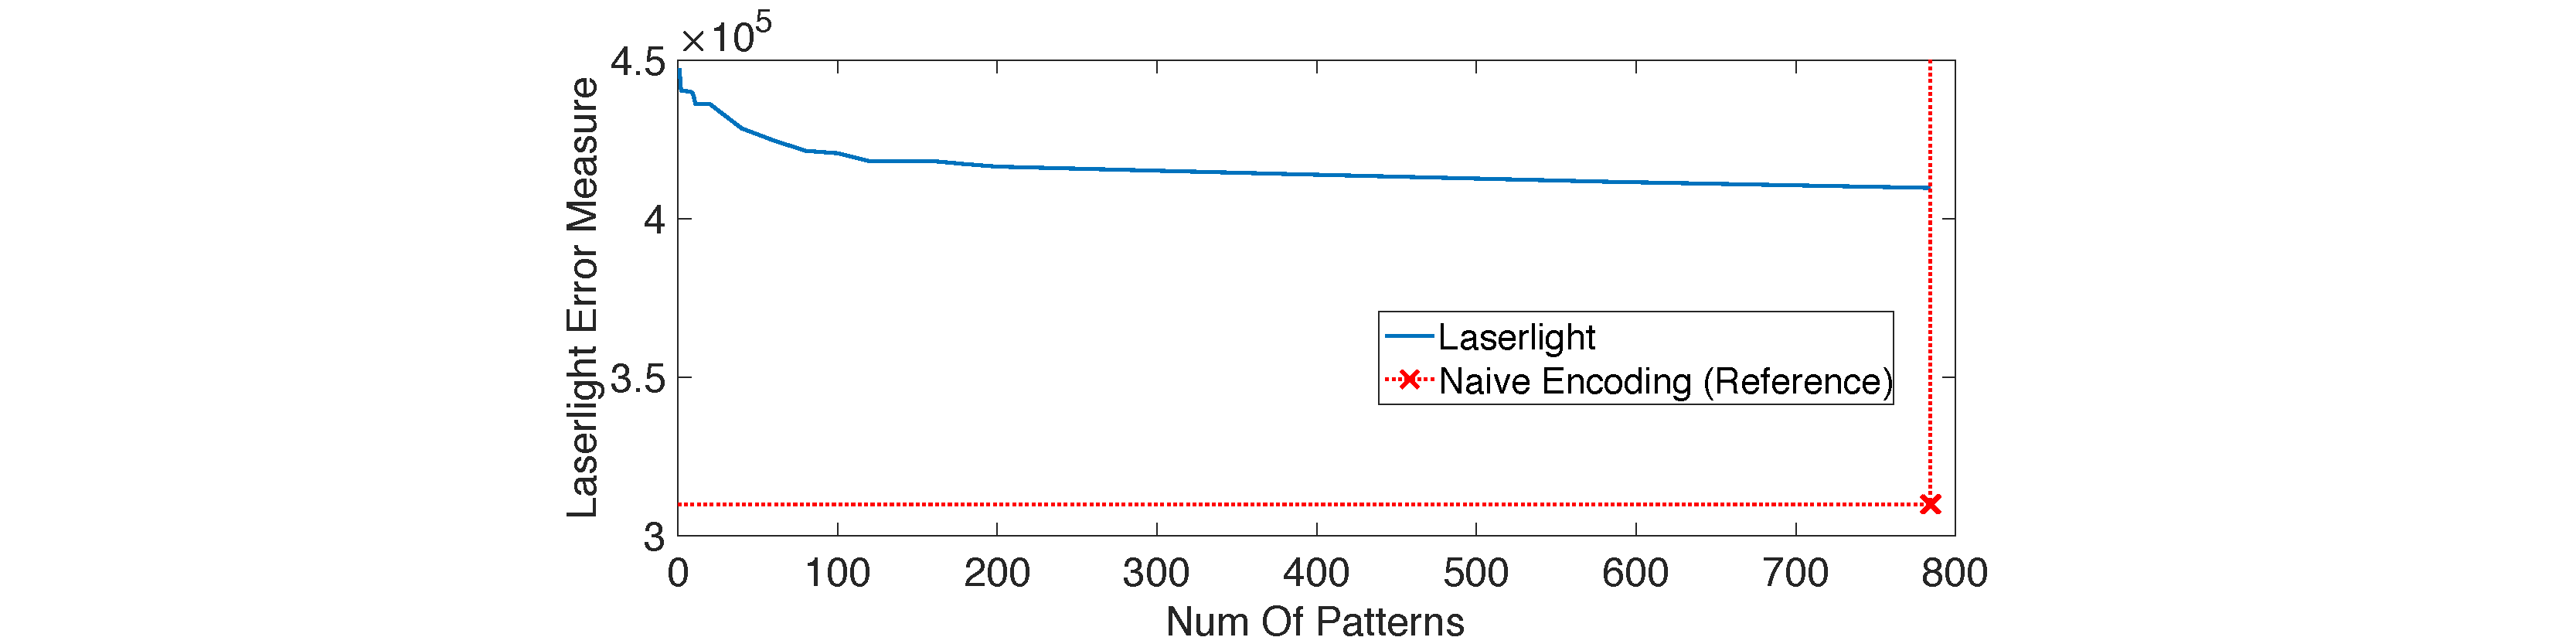
\includegraphics[width=\textwidth]{QueryLogSummarization/graphics/Laserlight_Error_vs_NumOfPatterns.pdf}
        \bfcaption{Laserlight Error v. \# of Patterns on Income data}
        \label{fig:Laserlight_Error_vs_NumOfPatterns}
    \end{subfigure}
    ~
    \begin{subfigure}[b]{0.48\textwidth}
        \centering       
        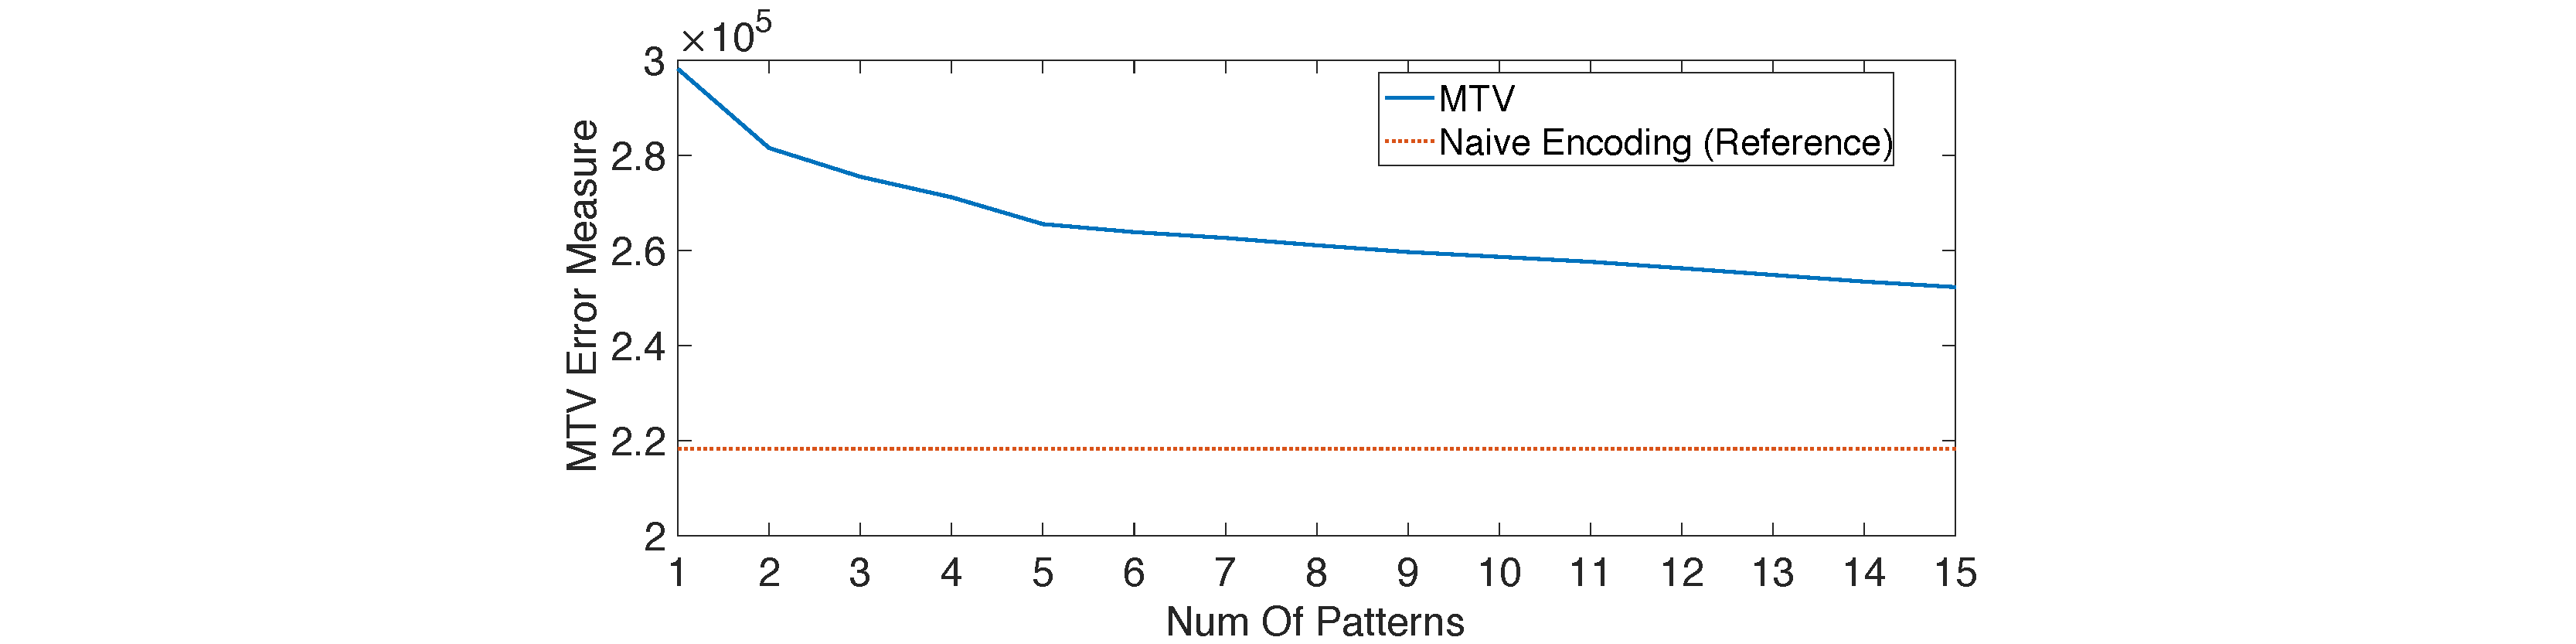
\includegraphics[width=\textwidth]{QueryLogSummarization/graphics/MTV_Error_vs_NumOfPatterns.pdf}
        \bfcaption{MTV Error v. \# of Patterns on Mushroom data}     
        \label{fig:MTV_Error_vs_NumOfPatterns}
    \end{subfigure}
    ~
    \bfcaption{Error v. Number of Patterns. Note: non-zero start of y-axis.}   
    \label{fig:performance_vs_num_of_patterns}
    \trimfigurewhitespace
\end{figure}

\subsubsection{Classical Laserlight and MTV}
\label{sec:classicallaserlightandmtv}

\tinysection{Establishing Baselines} 
To establish baselines, we evaluate \textit{Laserlight} and \textit{MTV} on their own data sets.
The take-aways from related experiments are that (1) \textit{naive encoding} is faster and more accurate than classical \textit{Laserlight} and \textit{MTV}; (2) the runtime increases superlinearly with the number of patterns mined from both \textit{Laserlight} and \textit{MTV}.

\tinysection{Dimentionality Reduction}
Recall in Section~\ref{sec:refiningnaivemixtureencodings} that \textit{Laserlight} is restricted to $100$ features.
For its own \textit{Income} data set, \textit{Laserlight} can be applied with its full set of $783$ features.
This is due to the prior knowledge that the $783$ features belong to $9$ groups.
In each group, features are mutually exclusive which can be reduced to a single feature.
Similarly, \textit{Mushroom} data set can be reduced from $95$ to $21$ features (See Table~\ref{table:extendeddatasummary}).

The results related to Error measures are given in Figure~\ref{fig:performance_vs_num_of_patterns}.
X-axis is the number of patterns and y-axis represents the Error measure of \textit{Laserlight} and \textit{MTV} in Figure~\ref{fig:Laserlight_Error_vs_NumOfPatterns} and~\ref{fig:MTV_Error_vs_NumOfPatterns} respectively.
We incorporate \textit{naive encoding} in Figure~\ref{fig:Laserlight_Error_vs_NumOfPatterns} as the reference method.
Since there are $784$ total number of features for \textit{Income} data set, the verbosity of \textit{naive encoding} will be $784$, which is shown as vertical dotted line in Figure~\ref{fig:Laserlight_Error_vs_NumOfPatterns}.
For \textit{Mushroom} data set, the verbosity of its \textit{naive encoding} will be $96$.
However, \textit{MTV} quits with error message if it is requested to mine over $15$ patterns.
Hence for Figure~\ref{fig:MTV_Error_vs_NumOfPatterns}, the limit of x-axis is $15$ and we only show Error of \textit{naive encoding} as a reference line without marking out its verbosity. 
We observe in Figure~\ref{fig:Laserlight_Error_vs_NumOfPatterns} that \textit{naive encoding} outperforms \textit{Laserlight} when their verbosity is equal (i.e., $784$).
In addition, after $100$ patterns, the slope of Error reduction becomes relatively flat.
Similar observation can be made from Figure~\ref{fig:MTV_Error_vs_NumOfPatterns}.

\begin{figure}[h!]
	\captionsetup[subfigure]{justification=centering}
    \centering

    \begin{subfigure}[b]{0.48\textwidth}
        \centering       
        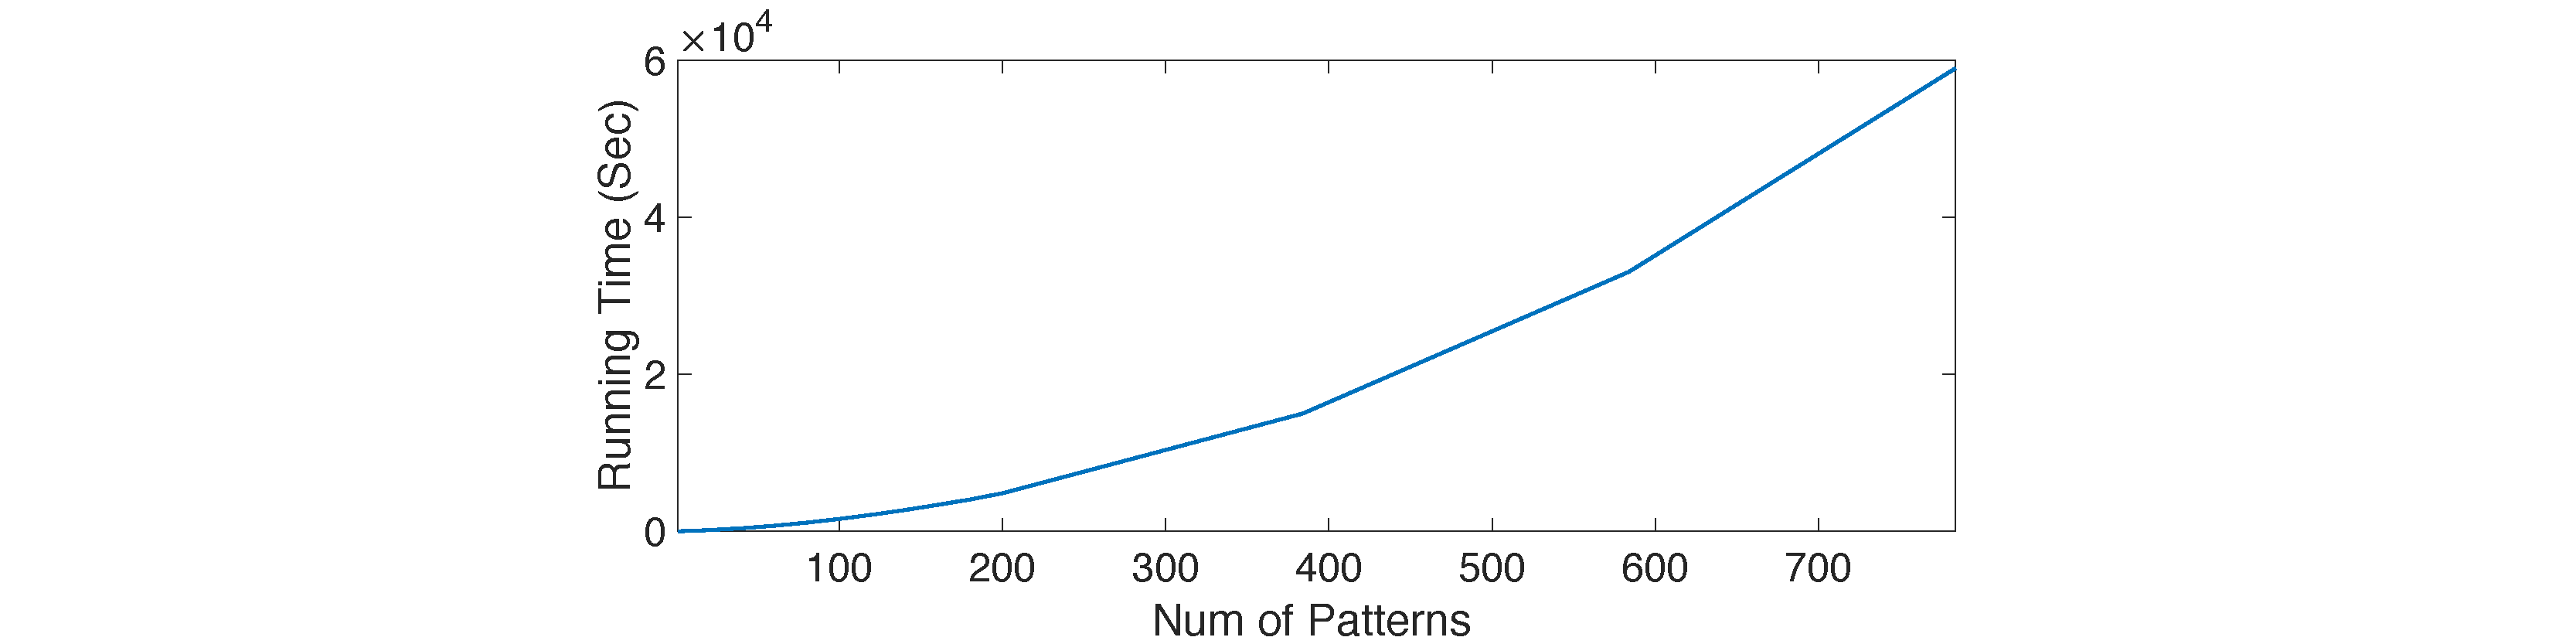
\includegraphics[width=\textwidth]{QueryLogSummarization/graphics/Laserlight_runningTimes_vs_NumOfPatterns.pdf}
 \bfcaption{Laserlight Running Time on Income Data}      \label{fig:laserlight_runningTimes_vs_NumOfPatterns}
\end{subfigure}
    ~
     \begin{subfigure}[b]{0.48\textwidth}
        \centering       
        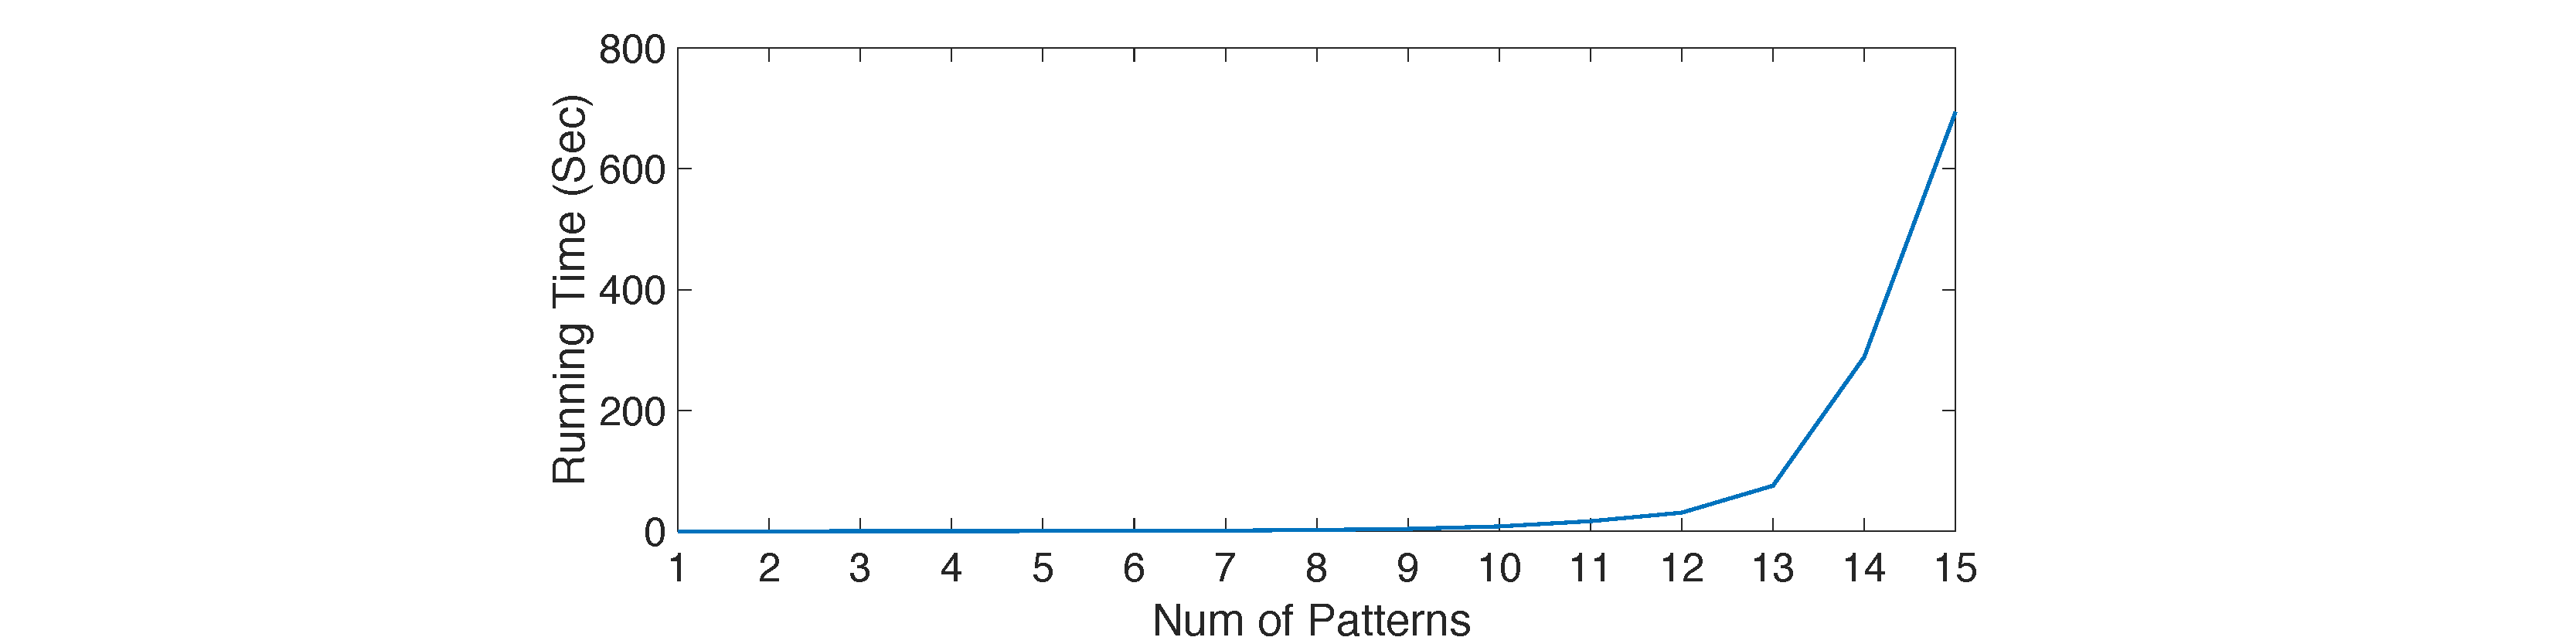
\includegraphics[width=\textwidth]{QueryLogSummarization/graphics/MTV_runningTimes_vs_NumOfPatterns.pdf}
 \bfcaption{MTV Running Time on Mushroom data}      \label{fig:mtv_runningTimes_vs_NumOfPatterns}
\end{subfigure}
    ~   
\bfcaption{Running Time of Laserlight and MTV}   \label{fig:runningTime_analysis}
\trimfigurewhitespace
\end{figure}

Next I show corresponding run time results in Figure~\ref{fig:runningTime_analysis}.
We observe that the running time increases exponentially with the number of patterns, for both \textit{Laserlight} and \textit{MTV}.

\subsubsection{Generalizing Laserlight and MTV}
\label{sec:generalizinglaserlightandmtv}
In this section, we generalize \textit{Laserlight} and \textit{MTV} on partitioned data by applying them on each cluster.
We then combine Errors on all clusters by taking a weighted average, as described in Section~\ref{sec:generalizedinformationlossmeasures}.
Depending on how many patterns are mined from each cluster, \textit{Laserlight} and \textit{MTV} can be generalized into two types: (1) The number of patterns mined from each cluster is scaled to be equal to Verbosity of the \emph{naive encoding}; and (2) The total number of patterns mined from all clusters is fixed to a given number.
I name the first type \emph{Laserlight (MTV) Mixture Scaled}, which is comparable to \emph{naive mixture encoding}.
I name the second type \emph{Laserlight (MTV) Mixture Fixed}, which is comparable to the classical \emph{LaserLight (MTV)} algorithm.

\tinysection{Take-away}
As the data is partitioned into more clusters, both runtime and Error of \emph{Laserlight (MTV) Mixture Fixed} exponentially decrease.
This observation can be potentially generalized to other pattern mining algorithms.
For experiment details, I refer the reader to~\cite{DBLP:journals/corr/abs-1809-00405}.

\begin{figure}[h!]
	\captionsetup[subfigure]{justification=centering}
    \centering
    \begin{subfigure}[b]{0.47\textwidth}
        \centering       
        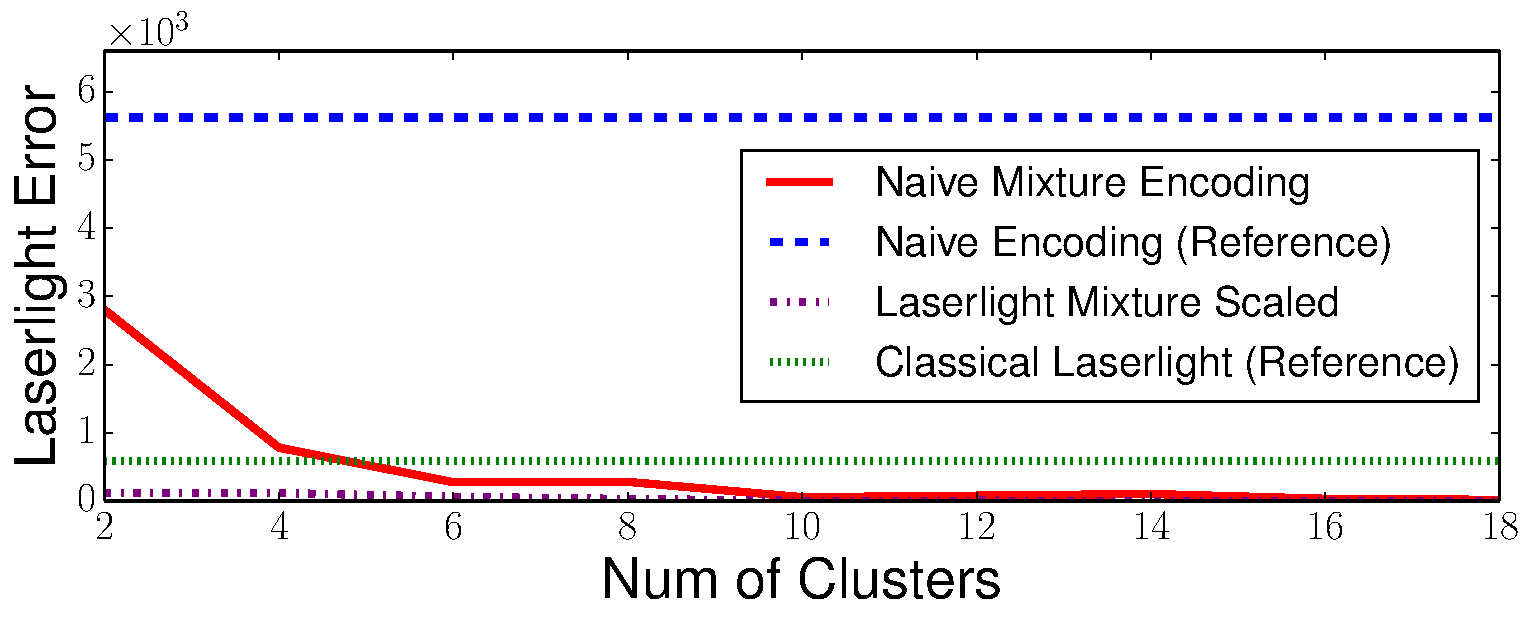
\includegraphics[width=\textwidth]{QueryLogSummarization/graphics/Laserlight_Errors_vs_NumOfClusters.pdf}
 \bfcaption{Laserlight Error v. \# of Clusters on Mushroom data}      \label{fig:LaserlightMixture_Errors_vs_NumOfClusters}
\end{subfigure}
    ~
\begin{subfigure}[b]{0.47\textwidth}
  \centering       
  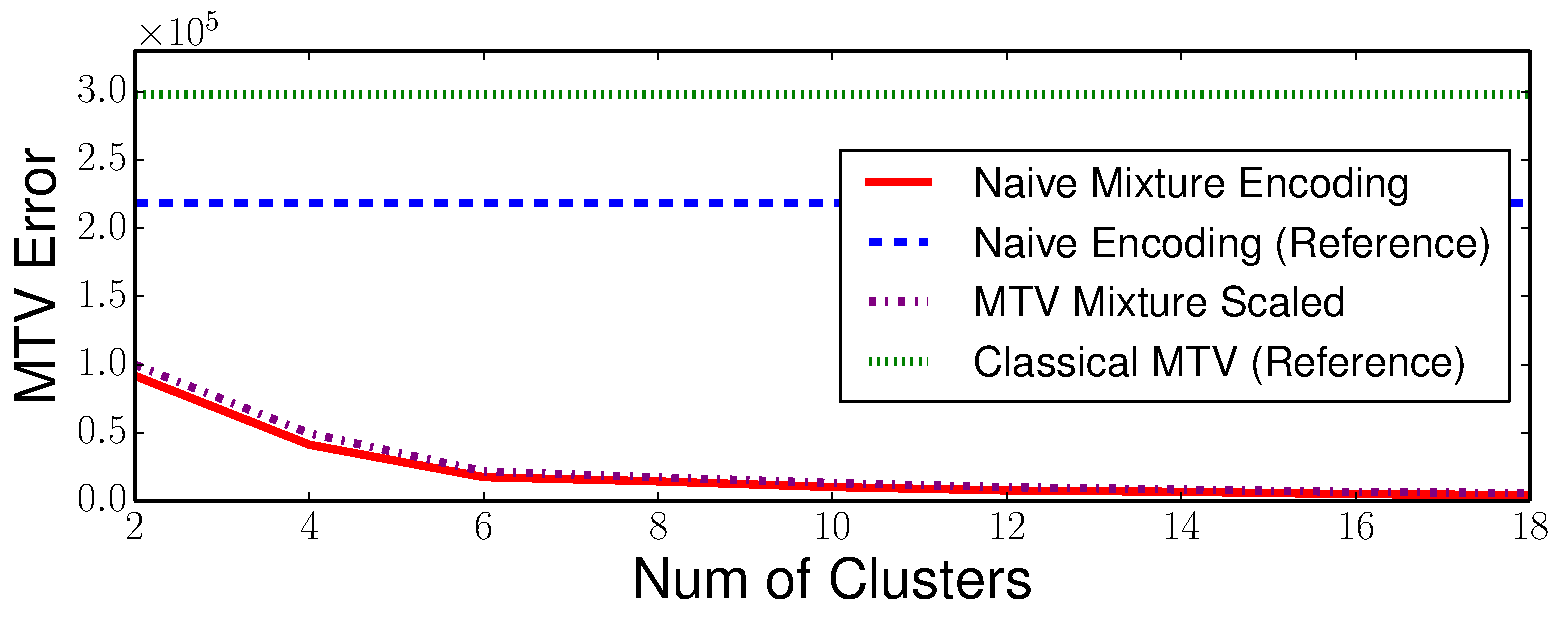
\includegraphics[width=\textwidth]{QueryLogSummarization/graphics/MTV_Error_vs_NumOfClusters.pdf}
 \bfcaption{MTV Error v. \# of Clusters on Mushroom data}     
 \label{fig:MTVMixture_vs_Laserlight_runningTimes_IncomeData}
\end{subfigure}
~
\bfcaption{Naive Mixture v. Laserlight/MTV Mixture}   
\label{fig:Naive Mixture Encoding_vs_Laserlight&MTV_Mixture}
\trimfigurewhitespace
\end{figure}
\subsubsection{Comparison with Naive Mixture Encoding}
\label{sec:Evaluating_Naive_Mixture_Encoding}

At last, we compare \emph{Laserlight (MTV) Mixture Scaled} with \emph{naive mixture encoding}.
Note that it is time-consuming for \emph{Laserlight} to mine the same number of patterns as \emph{naive encoding} on \emph{Income} data (See runtime analysis in~\cite{DBLP:journals/corr/abs-1809-00405}), I choose \emph{Mushroom} data for \emph{Laserlight Mixture Scaled} instead.
The experiment results are given in Figure~\ref{fig:Naive Mixture Encoding_vs_Laserlight&MTV_Mixture}. 
The x-axis for all sub-figures in Figure~\ref{fig:Naive Mixture Encoding_vs_Laserlight&MTV_Mixture} represents the number of clusters and the y-axes stands for \emph{Laserlight} and \emph{MTV} Error respectively.
I incorporate baselines (i.e., \emph{naive encoding}, classical \emph{Laserlight} and \emph{MTV}) as reference lines in Figure~\ref{fig:LaserlightMixture_Errors_vs_NumOfClusters} and~\ref{fig:MTVMixture_vs_Laserlight_runningTimes_IncomeData} respectively.
We also experienced a limitation of $15$ patterns for \emph{MTV}.
Hence the comparison between \emph{MTV Mixture Scaled} and {naive mixture encoding} is not strictly on equal footing as \emph{MTV Mixture Scaled} is not able to reach the same Total Verbosity as \emph{naive mixture encoding}.
Note that their difference in Verbosity is mitigated by the fact that \emph{MTV} Error measure penalizes encoding Verbosity.

Figure~\ref{fig:LaserlightMixture_Errors_vs_NumOfClusters} shows that both \emph{naive mixture encoding} and \emph{Laserlight Mixture Scaled} have lower Error than their baselines.
In addition, \emph{Laserlight Mixture Scaled} has lower Error than \emph{naive mixture encoding} when the number of clusters is less than $4$ and they become close after $6$ clusters.
In other words, \emph{Laserlight} is more accurate on lightly partitioned data. 
As the data is further partitioned, clusters become easier to summarize, and \emph{naive encoding} becomes more similar to \emph{Laserlight}.
Figure~\ref{fig:MTVMixture_vs_Laserlight_runningTimes_IncomeData} shows that \emph{naive mixture encoding} marginally outperforms \emph{MTV Mixture Scaled}.

\tinysection{Take-away}
\emph{Naive mixture encoding} is faster and has similar (lower) Error than \emph{Laserlight (MTV) Mixture Scaled}.
